\documentclass{article} % For LaTeX2e
\usepackage{icomp2024_conference,times}

% Optional math command from https://github.com/goodfeli/dlbook_notation.
%%%%% NEW MATH DEFINITIONS %%%%%

\usepackage{amsmath,amsfonts,bm}

% Mark sections of captions for referring to divisions of figures
\newcommand{\figleft}{{\em (Left)}}
\newcommand{\figcenter}{{\em (Center)}}
\newcommand{\figright}{{\em (Right)}}
\newcommand{\figtop}{{\em (Top)}}
\newcommand{\figbottom}{{\em (Bottom)}}
\newcommand{\captiona}{{\em (a)}}
\newcommand{\captionb}{{\em (b)}}
\newcommand{\captionc}{{\em (c)}}
\newcommand{\captiond}{{\em (d)}}

% Highlight a newly defined term
\newcommand{\newterm}[1]{{\bf #1}}


% Figure reference, lower-case.
\def\figref#1{figure~\ref{#1}}
% Figure reference, capital. For start of sentence
\def\Figref#1{Figure~\ref{#1}}
\def\twofigref#1#2{figures \ref{#1} and \ref{#2}}
\def\quadfigref#1#2#3#4{figures \ref{#1}, \ref{#2}, \ref{#3} and \ref{#4}}
% Section reference, lower-case.
\def\secref#1{section~\ref{#1}}
% Section reference, capital.
\def\Secref#1{Section~\ref{#1}}
% Reference to two sections.
\def\twosecrefs#1#2{sections \ref{#1} and \ref{#2}}
% Reference to three sections.
\def\secrefs#1#2#3{sections \ref{#1}, \ref{#2} and \ref{#3}}
% Reference to an equation, lower-case.
\def\eqref#1{equation~\ref{#1}}
% Reference to an equation, upper case
\def\Eqref#1{Equation~\ref{#1}}
% A raw reference to an equation---avoid using if possible
\def\plaineqref#1{\ref{#1}}
% Reference to a chapter, lower-case.
\def\chapref#1{chapter~\ref{#1}}
% Reference to an equation, upper case.
\def\Chapref#1{Chapter~\ref{#1}}
% Reference to a range of chapters
\def\rangechapref#1#2{chapters\ref{#1}--\ref{#2}}
% Reference to an algorithm, lower-case.
\def\algref#1{algorithm~\ref{#1}}
% Reference to an algorithm, upper case.
\def\Algref#1{Algorithm~\ref{#1}}
\def\twoalgref#1#2{algorithms \ref{#1} and \ref{#2}}
\def\Twoalgref#1#2{Algorithms \ref{#1} and \ref{#2}}
% Reference to a part, lower case
\def\partref#1{part~\ref{#1}}
% Reference to a part, upper case
\def\Partref#1{Part~\ref{#1}}
\def\twopartref#1#2{parts \ref{#1} and \ref{#2}}

\def\ceil#1{\lceil #1 \rceil}
\def\floor#1{\lfloor #1 \rfloor}
\def\1{\bm{1}}
\newcommand{\train}{\mathcal{D}}
\newcommand{\valid}{\mathcal{D_{\mathrm{valid}}}}
\newcommand{\test}{\mathcal{D_{\mathrm{test}}}}

\def\eps{{\epsilon}}


% Random variables
\def\reta{{\textnormal{$\eta$}}}
\def\ra{{\textnormal{a}}}
\def\rb{{\textnormal{b}}}
\def\rc{{\textnormal{c}}}
\def\rd{{\textnormal{d}}}
\def\re{{\textnormal{e}}}
\def\rf{{\textnormal{f}}}
\def\rg{{\textnormal{g}}}
\def\rh{{\textnormal{h}}}
\def\ri{{\textnormal{i}}}
\def\rj{{\textnormal{j}}}
\def\rk{{\textnormal{k}}}
\def\rl{{\textnormal{l}}}
% rm is already a command, just don't name any random variables m
\def\rn{{\textnormal{n}}}
\def\ro{{\textnormal{o}}}
\def\rp{{\textnormal{p}}}
\def\rq{{\textnormal{q}}}
\def\rr{{\textnormal{r}}}
\def\rs{{\textnormal{s}}}
\def\rt{{\textnormal{t}}}
\def\ru{{\textnormal{u}}}
\def\rv{{\textnormal{v}}}
\def\rw{{\textnormal{w}}}
\def\rx{{\textnormal{x}}}
\def\ry{{\textnormal{y}}}
\def\rz{{\textnormal{z}}}

% Random vectors
\def\rvepsilon{{\mathbf{\epsilon}}}
\def\rvtheta{{\mathbf{\theta}}}
\def\rva{{\mathbf{a}}}
\def\rvb{{\mathbf{b}}}
\def\rvc{{\mathbf{c}}}
\def\rvd{{\mathbf{d}}}
\def\rve{{\mathbf{e}}}
\def\rvf{{\mathbf{f}}}
\def\rvg{{\mathbf{g}}}
\def\rvh{{\mathbf{h}}}
\def\rvu{{\mathbf{i}}}
\def\rvj{{\mathbf{j}}}
\def\rvk{{\mathbf{k}}}
\def\rvl{{\mathbf{l}}}
\def\rvm{{\mathbf{m}}}
\def\rvn{{\mathbf{n}}}
\def\rvo{{\mathbf{o}}}
\def\rvp{{\mathbf{p}}}
\def\rvq{{\mathbf{q}}}
\def\rvr{{\mathbf{r}}}
\def\rvs{{\mathbf{s}}}
\def\rvt{{\mathbf{t}}}
\def\rvu{{\mathbf{u}}}
\def\rvv{{\mathbf{v}}}
\def\rvw{{\mathbf{w}}}
\def\rvx{{\mathbf{x}}}
\def\rvy{{\mathbf{y}}}
\def\rvz{{\mathbf{z}}}

% Elements of random vectors
\def\erva{{\textnormal{a}}}
\def\ervb{{\textnormal{b}}}
\def\ervc{{\textnormal{c}}}
\def\ervd{{\textnormal{d}}}
\def\erve{{\textnormal{e}}}
\def\ervf{{\textnormal{f}}}
\def\ervg{{\textnormal{g}}}
\def\ervh{{\textnormal{h}}}
\def\ervi{{\textnormal{i}}}
\def\ervj{{\textnormal{j}}}
\def\ervk{{\textnormal{k}}}
\def\ervl{{\textnormal{l}}}
\def\ervm{{\textnormal{m}}}
\def\ervn{{\textnormal{n}}}
\def\ervo{{\textnormal{o}}}
\def\ervp{{\textnormal{p}}}
\def\ervq{{\textnormal{q}}}
\def\ervr{{\textnormal{r}}}
\def\ervs{{\textnormal{s}}}
\def\ervt{{\textnormal{t}}}
\def\ervu{{\textnormal{u}}}
\def\ervv{{\textnormal{v}}}
\def\ervw{{\textnormal{w}}}
\def\ervx{{\textnormal{x}}}
\def\ervy{{\textnormal{y}}}
\def\ervz{{\textnormal{z}}}

% Random matrices
\def\rmA{{\mathbf{A}}}
\def\rmB{{\mathbf{B}}}
\def\rmC{{\mathbf{C}}}
\def\rmD{{\mathbf{D}}}
\def\rmE{{\mathbf{E}}}
\def\rmF{{\mathbf{F}}}
\def\rmG{{\mathbf{G}}}
\def\rmH{{\mathbf{H}}}
\def\rmI{{\mathbf{I}}}
\def\rmJ{{\mathbf{J}}}
\def\rmK{{\mathbf{K}}}
\def\rmL{{\mathbf{L}}}
\def\rmM{{\mathbf{M}}}
\def\rmN{{\mathbf{N}}}
\def\rmO{{\mathbf{O}}}
\def\rmP{{\mathbf{P}}}
\def\rmQ{{\mathbf{Q}}}
\def\rmR{{\mathbf{R}}}
\def\rmS{{\mathbf{S}}}
\def\rmT{{\mathbf{T}}}
\def\rmU{{\mathbf{U}}}
\def\rmV{{\mathbf{V}}}
\def\rmW{{\mathbf{W}}}
\def\rmX{{\mathbf{X}}}
\def\rmY{{\mathbf{Y}}}
\def\rmZ{{\mathbf{Z}}}

% Elements of random matrices
\def\ermA{{\textnormal{A}}}
\def\ermB{{\textnormal{B}}}
\def\ermC{{\textnormal{C}}}
\def\ermD{{\textnormal{D}}}
\def\ermE{{\textnormal{E}}}
\def\ermF{{\textnormal{F}}}
\def\ermG{{\textnormal{G}}}
\def\ermH{{\textnormal{H}}}
\def\ermI{{\textnormal{I}}}
\def\ermJ{{\textnormal{J}}}
\def\ermK{{\textnormal{K}}}
\def\ermL{{\textnormal{L}}}
\def\ermM{{\textnormal{M}}}
\def\ermN{{\textnormal{N}}}
\def\ermO{{\textnormal{O}}}
\def\ermP{{\textnormal{P}}}
\def\ermQ{{\textnormal{Q}}}
\def\ermR{{\textnormal{R}}}
\def\ermS{{\textnormal{S}}}
\def\ermT{{\textnormal{T}}}
\def\ermU{{\textnormal{U}}}
\def\ermV{{\textnormal{V}}}
\def\ermW{{\textnormal{W}}}
\def\ermX{{\textnormal{X}}}
\def\ermY{{\textnormal{Y}}}
\def\ermZ{{\textnormal{Z}}}

% Vectors
\def\vzero{{\bm{0}}}
\def\vone{{\bm{1}}}
\def\vmu{{\bm{\mu}}}
\def\vtheta{{\bm{\theta}}}
\def\va{{\bm{a}}}
\def\vb{{\bm{b}}}
\def\vc{{\bm{c}}}
\def\vd{{\bm{d}}}
\def\ve{{\bm{e}}}
\def\vf{{\bm{f}}}
\def\vg{{\bm{g}}}
\def\vh{{\bm{h}}}
\def\vi{{\bm{i}}}
\def\vj{{\bm{j}}}
\def\vk{{\bm{k}}}
\def\vl{{\bm{l}}}
\def\vm{{\bm{m}}}
\def\vn{{\bm{n}}}
\def\vo{{\bm{o}}}
\def\vp{{\bm{p}}}
\def\vq{{\bm{q}}}
\def\vr{{\bm{r}}}
\def\vs{{\bm{s}}}
\def\vt{{\bm{t}}}
\def\vu{{\bm{u}}}
\def\vv{{\bm{v}}}
\def\vw{{\bm{w}}}
\def\vx{{\bm{x}}}
\def\vy{{\bm{y}}}
\def\vz{{\bm{z}}}

% Elements of vectors
\def\evalpha{{\alpha}}
\def\evbeta{{\beta}}
\def\evepsilon{{\epsilon}}
\def\evlambda{{\lambda}}
\def\evomega{{\omega}}
\def\evmu{{\mu}}
\def\evpsi{{\psi}}
\def\evsigma{{\sigma}}
\def\evtheta{{\theta}}
\def\eva{{a}}
\def\evb{{b}}
\def\evc{{c}}
\def\evd{{d}}
\def\eve{{e}}
\def\evf{{f}}
\def\evg{{g}}
\def\evh{{h}}
\def\evi{{i}}
\def\evj{{j}}
\def\evk{{k}}
\def\evl{{l}}
\def\evm{{m}}
\def\evn{{n}}
\def\evo{{o}}
\def\evp{{p}}
\def\evq{{q}}
\def\evr{{r}}
\def\evs{{s}}
\def\evt{{t}}
\def\evu{{u}}
\def\evv{{v}}
\def\evw{{w}}
\def\evx{{x}}
\def\evy{{y}}
\def\evz{{z}}

% Matrix
\def\mA{{\bm{A}}}
\def\mB{{\bm{B}}}
\def\mC{{\bm{C}}}
\def\mD{{\bm{D}}}
\def\mE{{\bm{E}}}
\def\mF{{\bm{F}}}
\def\mG{{\bm{G}}}
\def\mH{{\bm{H}}}
\def\mI{{\bm{I}}}
\def\mJ{{\bm{J}}}
\def\mK{{\bm{K}}}
\def\mL{{\bm{L}}}
\def\mM{{\bm{M}}}
\def\mN{{\bm{N}}}
\def\mO{{\bm{O}}}
\def\mP{{\bm{P}}}
\def\mQ{{\bm{Q}}}
\def\mR{{\bm{R}}}
\def\mS{{\bm{S}}}
\def\mT{{\bm{T}}}
\def\mU{{\bm{U}}}
\def\mV{{\bm{V}}}
\def\mW{{\bm{W}}}
\def\mX{{\bm{X}}}
\def\mY{{\bm{Y}}}
\def\mZ{{\bm{Z}}}
\def\mBeta{{\bm{\beta}}}
\def\mPhi{{\bm{\Phi}}}
\def\mLambda{{\bm{\Lambda}}}
\def\mSigma{{\bm{\Sigma}}}

% Tensor
\DeclareMathAlphabet{\mathsfit}{\encodingdefault}{\sfdefault}{m}{sl}
\SetMathAlphabet{\mathsfit}{bold}{\encodingdefault}{\sfdefault}{bx}{n}
\newcommand{\tens}[1]{\bm{\mathsfit{#1}}}
\def\tA{{\tens{A}}}
\def\tB{{\tens{B}}}
\def\tC{{\tens{C}}}
\def\tD{{\tens{D}}}
\def\tE{{\tens{E}}}
\def\tF{{\tens{F}}}
\def\tG{{\tens{G}}}
\def\tH{{\tens{H}}}
\def\tI{{\tens{I}}}
\def\tJ{{\tens{J}}}
\def\tK{{\tens{K}}}
\def\tL{{\tens{L}}}
\def\tM{{\tens{M}}}
\def\tN{{\tens{N}}}
\def\tO{{\tens{O}}}
\def\tP{{\tens{P}}}
\def\tQ{{\tens{Q}}}
\def\tR{{\tens{R}}}
\def\tS{{\tens{S}}}
\def\tT{{\tens{T}}}
\def\tU{{\tens{U}}}
\def\tV{{\tens{V}}}
\def\tW{{\tens{W}}}
\def\tX{{\tens{X}}}
\def\tY{{\tens{Y}}}
\def\tZ{{\tens{Z}}}


% Graph
\def\gA{{\mathcal{A}}}
\def\gB{{\mathcal{B}}}
\def\gC{{\mathcal{C}}}
\def\gD{{\mathcal{D}}}
\def\gE{{\mathcal{E}}}
\def\gF{{\mathcal{F}}}
\def\gG{{\mathcal{G}}}
\def\gH{{\mathcal{H}}}
\def\gI{{\mathcal{I}}}
\def\gJ{{\mathcal{J}}}
\def\gK{{\mathcal{K}}}
\def\gL{{\mathcal{L}}}
\def\gM{{\mathcal{M}}}
\def\gN{{\mathcal{N}}}
\def\gO{{\mathcal{O}}}
\def\gP{{\mathcal{P}}}
\def\gQ{{\mathcal{Q}}}
\def\gR{{\mathcal{R}}}
\def\gS{{\mathcal{S}}}
\def\gT{{\mathcal{T}}}
\def\gU{{\mathcal{U}}}
\def\gV{{\mathcal{V}}}
\def\gW{{\mathcal{W}}}
\def\gX{{\mathcal{X}}}
\def\gY{{\mathcal{Y}}}
\def\gZ{{\mathcal{Z}}}

% Sets
\def\sA{{\mathbb{A}}}
\def\sB{{\mathbb{B}}}
\def\sC{{\mathbb{C}}}
\def\sD{{\mathbb{D}}}
% Don't use a set called E, because this would be the same as our symbol
% for expectation.
\def\sF{{\mathbb{F}}}
\def\sG{{\mathbb{G}}}
\def\sH{{\mathbb{H}}}
\def\sI{{\mathbb{I}}}
\def\sJ{{\mathbb{J}}}
\def\sK{{\mathbb{K}}}
\def\sL{{\mathbb{L}}}
\def\sM{{\mathbb{M}}}
\def\sN{{\mathbb{N}}}
\def\sO{{\mathbb{O}}}
\def\sP{{\mathbb{P}}}
\def\sQ{{\mathbb{Q}}}
\def\sR{{\mathbb{R}}}
\def\sS{{\mathbb{S}}}
\def\sT{{\mathbb{T}}}
\def\sU{{\mathbb{U}}}
\def\sV{{\mathbb{V}}}
\def\sW{{\mathbb{W}}}
\def\sX{{\mathbb{X}}}
\def\sY{{\mathbb{Y}}}
\def\sZ{{\mathbb{Z}}}

% Entries of a matrix
\def\emLambda{{\Lambda}}
\def\emA{{A}}
\def\emB{{B}}
\def\emC{{C}}
\def\emD{{D}}
\def\emE{{E}}
\def\emF{{F}}
\def\emG{{G}}
\def\emH{{H}}
\def\emI{{I}}
\def\emJ{{J}}
\def\emK{{K}}
\def\emL{{L}}
\def\emM{{M}}
\def\emN{{N}}
\def\emO{{O}}
\def\emP{{P}}
\def\emQ{{Q}}
\def\emR{{R}}
\def\emS{{S}}
\def\emT{{T}}
\def\emU{{U}}
\def\emV{{V}}
\def\emW{{W}}
\def\emX{{X}}
\def\emY{{Y}}
\def\emZ{{Z}}
\def\emSigma{{\Sigma}}

% entries of a tensor
% Same font as tensor, without \bm wrapper
\newcommand{\etens}[1]{\mathsfit{#1}}
\def\etLambda{{\etens{\Lambda}}}
\def\etA{{\etens{A}}}
\def\etB{{\etens{B}}}
\def\etC{{\etens{C}}}
\def\etD{{\etens{D}}}
\def\etE{{\etens{E}}}
\def\etF{{\etens{F}}}
\def\etG{{\etens{G}}}
\def\etH{{\etens{H}}}
\def\etI{{\etens{I}}}
\def\etJ{{\etens{J}}}
\def\etK{{\etens{K}}}
\def\etL{{\etens{L}}}
\def\etM{{\etens{M}}}
\def\etN{{\etens{N}}}
\def\etO{{\etens{O}}}
\def\etP{{\etens{P}}}
\def\etQ{{\etens{Q}}}
\def\etR{{\etens{R}}}
\def\etS{{\etens{S}}}
\def\etT{{\etens{T}}}
\def\etU{{\etens{U}}}
\def\etV{{\etens{V}}}
\def\etW{{\etens{W}}}
\def\etX{{\etens{X}}}
\def\etY{{\etens{Y}}}
\def\etZ{{\etens{Z}}}

% The true underlying data generating distribution
\newcommand{\pdata}{p_{\rm{data}}}
% The empirical distribution defined by the training set
\newcommand{\ptrain}{\hat{p}_{\rm{data}}}
\newcommand{\Ptrain}{\hat{P}_{\rm{data}}}
% The model distribution
\newcommand{\pmodel}{p_{\rm{model}}}
\newcommand{\Pmodel}{P_{\rm{model}}}
\newcommand{\ptildemodel}{\tilde{p}_{\rm{model}}}
% Stochastic autoencoder distributions
\newcommand{\pencode}{p_{\rm{encoder}}}
\newcommand{\pdecode}{p_{\rm{decoder}}}
\newcommand{\precons}{p_{\rm{reconstruct}}}

\newcommand{\laplace}{\mathrm{Laplace}} % Laplace distribution

\newcommand{\E}{\mathbb{E}}
\newcommand{\Ls}{\mathcal{L}}
\newcommand{\R}{\mathbb{R}}
\newcommand{\emp}{\tilde{p}}
\newcommand{\lr}{\alpha}
\newcommand{\reg}{\lambda}
\newcommand{\rect}{\mathrm{rectifier}}
\newcommand{\softmax}{\mathrm{softmax}}
\newcommand{\sigmoid}{\sigma}
\newcommand{\softplus}{\zeta}
\newcommand{\KL}{D_{\mathrm{KL}}}
\newcommand{\Var}{\mathrm{Var}}
\newcommand{\standarderror}{\mathrm{SE}}
\newcommand{\Cov}{\mathrm{Cov}}
% Wolfram Mathworld says $L^2$ is for function spaces and $\ell^2$ is for vectors
% But then they seem to use $L^2$ for vectors throughout the site, and so does
% wikipedia.
\newcommand{\normlzero}{L^0}
\newcommand{\normlone}{L^1}
\newcommand{\normltwo}{L^2}
\newcommand{\normlp}{L^p}
\newcommand{\normmax}{L^\infty}

\newcommand{\parents}{Pa} % See usage in notation.tex. Chosen to match Daphne's book.

\DeclareMathOperator*{\argmax}{arg\,max}
\DeclareMathOperator*{\argmin}{arg\,min}

\DeclareMathOperator{\sign}{sign}
\DeclareMathOperator{\Tr}{Tr}
\let\ab\allowbreak


\usepackage{hyperref}
\usepackage{url}
\usepackage{amsmath,amssymb}
\usepackage{amsthm}
\usepackage{algorithm}
\usepackage{algorithmic}
\usepackage{graphicx}
\usepackage{subcaption}
\newtheorem{lemma}{Lemma}
\newcommand{\norm}[1]{\lVert #1\rVert}


%\title{From Muon to Neon: Introducing Nuclear Norm to Large Matrices}
\title{The Nuclear Norm and Beyond: Dual Norms and Combinations for Matrix Optimization}

% Authors must not appear in the submitted version. They should be hidden
% as long as the \icompfinalcopy macro remains commented out below.
% Non-anonymous submissions will be rejected without review.

\author{Alexey Kravatskiy \\
Moscow Institute of Physics and Technology (MIPT) \\
\texttt{kravtskii.aiu@phystech.edu} \\
\And
Ivan Kozyrev \\
Moscow Institute of Physics and Technology (MIPT) \\
\texttt{kozyrev.in@phystech.edu} \\
\And
Nikolai Kozlov \\
Moscow Institute of Physics and Technology (MIPT) \\
\texttt{kozlov.na@phystech.edu} \\
\And
Alexander Vinogradov \\
Moscow Institute of Physics and Technology (MIPT) \\
\texttt{vinogradov.am@phystech.edu} \\
\And
Daniil Merkulov \\
Moscow Institute of Physics and Technology (MIPT), Skoltech, HSE, Sber \\
\texttt{daniil.merkulov@phystech.edu} \\
\And
Ivan Oseledets \\
AIRI, Skoltech \\
\texttt{i.oseledets@skoltech.ru}
}

% The \author macro works with any number of authors. There are two commands
% used to separate the names and addresses of multiple authors: \And and \AND.
%
% Using \And between authors leaves it to \LaTeX{} to determine where to break
% the lines. Using \AND forces a linebreak at that point. So, if \LaTeX{}
% puts 3 of 4 authors names on the first line, and the last on the second
% line, try using \AND instead of \And before the third author name.

\newcommand{\fix}{\marginpar{FIX}}
\newcommand{\new}{\marginpar{NEW}}

%\icompfinalcopy % Uncomment for camera-ready version, but NOT for submission.

%------------------------------------------------------------------------------------
% \epsilon is predefined; override to use \varepsilon
\renewcommand{\epsilon}{\varepsilon}
\newcommand{\Rmn}{\R^{m\times n}}
\newcommand{\cB}{\mathcal{B}}
\newcommand{\cD}{\mathcal{D}}
\newcommand{\cO}{\mathcal{O}}
\newcommand{\cS}{\mathcal{S}}
\newcommand{\Ed}[2]{\mathbb{E}_{#1}\left[#2\right]}
\usepackage{mathtools}
\DeclarePairedDelimiter{\sqne}{\|}{\|_2^2}
%\DeclarePairedDelimiter{\norme}{\|}{\|_2}
\DeclarePairedDelimiter{\normf}{\|}{\|_\mathrm{F}}
\DeclarePairedDelimiter{\normfstar}{\|}{\|_\mathrm{F*}}
\DeclarePairedDelimiter{\normftwo}{\|}{\|_\mathrm{F2}}
\DeclarePairedDelimiter{\sqns}{\|}{\|_{\mathrm{op}}^2}
\DeclarePairedDelimiter{\norms}{\|}{\|_{\mathrm{op}}}
\DeclarePairedDelimiter{\sqnn}{\|}{\|_{\mathrm{nuc}}^2}
\DeclarePairedDelimiter{\sqnf}{\|}{\|_{\mathrm{F}}^2}
\DeclarePairedDelimiter{\normn}{\|}{\|_{\mathrm{nuc}}}
\def\<#1,#2>{\langle #1,#2\rangle}
\DeclarePairedDelimiter{\dotprod}{\langle}{\rangle}

\usepackage{cleveref}
\usepackage{environ}
\newcounter{aequation}
\NewEnviron{aequation}{\refstepcounter{aequation}$$\BODY\eqno{\text{(A\theaequation)}}$$}
\crefname{aequation}{assumption}{assumptions}
\creflabelformat{aequation}{(#2A#1#3)}

\usepackage{amsmath}
\DeclareMathOperator{\tr}{tr}
\DeclareMathOperator{\diag}{diag}

%------------------------------------------------------------------------------------

\begin{document}


\maketitle

\begin{abstract}
In this article, we explore the use of matrix norms for optimizing functions of weight matrices, a crucial problem in training large language models. Moving beyond the spectral norm that underlies the Muon update, we leverage the nuclear norm, its affine combinations with other norms, and their corresponding duals to develop a new family of Muon-like algorithms. We complement our theoretical analysis with an extensive empirical study of the algorithms across a wide range of tasks and settings.
\end{abstract}


\section{Introduction}
 Minimizing loss functions in unprecedentedly high-dimensional spaces has recently become an integral and crucial part in training large language models. Hence, new scalable, time- and memory-efficient algorithms have been demanded. Besides well-known Adam and AdamW \cite{kingma2014adam}, \cite{loshchilov2017decoupled}, recently proposed Muon has shown promising results on different benchmarks (CIFAR, NanoGPT, citations). Its key difference from earlier algorthims is that it has been constructed specifically for optimizing functions of weight matrices. Such functions are common in modern machine learning (citations), so it does not significantly restrict Muon's applicability to modern problems.

 That is what can be said from a practical point of view. From the perspective of theory, Muon's main innovation was an intentional usage of matrix norms, i.e. the spectral norm, to derive the algorithm's update (cite Deriving Muon). Several other attempts have been since made to construct new algorithms, mainly generalizations of Muon's paradigm (\cite{pethick2025training} and \cite{riabinin2025gluon}).

 Based upon recent theoretical advances that explain some theory behind Muon, Scion and Gluon (\cite{bernstein2025deriving,kovalev2025understanding,pethick2025training,riabinin2025gluon}), we explore application of other matrix norms to optimization of functions of matrices. As it has been done with Muon, we stipulate that our algorithms' updates be fast to compute.
\iffalse
\begin{itemize}
    \item Hype of Muon and others:
    \begin{itemize}
        \item Importance of the functions of a matrix weight. Special structure.
        \item Write the equation
        \item Memory efficiency and hyperparameter transferability
        \item Proven efficient computing (cite benchmarks and Dion and Cosmos)
    \end{itemize}
    \item Comparison:
    \begin{itemize}
        \item Shampoo (very compute intensive for large layers, we need asymptotics!), second order
        \item LMO has produced several effective algorithms: Muon, Dion, Scion, Gluon (citations)
        \item generalization is better for Muon and others (citations!). Possibly nuSAM here (definitely)
        \item Scion and Gluon for multilayer
        \item Gluon for (L0, L1)-smooth problems, which is more realistic (low L0, faster convergence - no impractically small stepsizes)
    \end{itemize}
    \item Analyis:
    \begin{itemize}
        \item Several generalizations have been already presented by the community: Old Optimizer and New Norm (idea and evidence that it explains famous algorithms); Pethick (LMO and different layers); Kovalev (as trust region and arbitrary norm); Gluon (generalized smoothness model).
        \item However, to the best of our knowledge, no attempt has been made to try other norms. Here we come in.
        \item No attempt to mitigate high computation cost of matrix computation has been made. Here again we come in.
        \item It has been shown that $O(1/esp^4)$ bounds for Muon, Scion, Gluon and even Adam for L-smooth functions (citations). Some bounds depend on the dimensionality of space (cite Kovalev), which for spectral norm gives much more iterations (cite Kovalev)
        \item This motivates us to try new norms
    \end{itemize}
\end{itemize}
\fi


\section{Problem Statement}
\subsection{Function of a matrix and Assumptions}
    Warning: the text was copied, while formulas were adapted. We need to rephrase the subsection! 
    We consider the problem of minimizing a differentiable matrix function $F(\cdot)\colon \Rmn \to \R$
    \begin{equation}\label{eq:mat}
        \min_{\mX \in \Rmn} f(\mX).
    \end{equation}

    To make the theoretical analysis possible in the future, we make three reasonable non-restrictive assumptions.
    Idea: move gradient assumptions and smoothness to the L-smooth part. Here we need only custom norm and their relation to the Frobenius norm.

{\bf Stochastic gradient estimator.}
    We assume access to a stochastic estimator $g(\cdot\,;\xi)\colon \Rmn \to \Rmn$ of the gradient $\nabla f(\cdot)$, where $\xi \sim \cD$ is a random variable sampled from a probability distribution $\cD$. We assume that the stochastic gradient estimator $g(\cdot;\xi)$ is unbiased and has bounded variance, that is, the following relations hold:
    \begin{aequation}\label{eq:variance}
    \Ed{\xi \sim \cD}{g(\mX;\xi)} = \nabla f(\mX)
    \quad\text{and}\quad
    \Ed{\xi \sim \cD}{\sqnf{g(\mX;\xi) - \nabla f(\mX)}} \leq \sigma^2
    \quad\text{for all}\;
    \mX \in \Rmn,
    \end{aequation}
    where $\sigma > 0$ is a positive variance parameter, and $\normf{\cdot}$ is the standard Euclidean, i.e. Frobenius, norm induced by the inner product $\<\cdot,\cdot>$, i.e., $\normf{\mX} = \sqrt{\<\mX,\mX>}=\sqrt{\tr(\mX^\top \mX)}$. These assumptions have been widely adopted for the analysis of many stochastic gradient optimization algorithms \citep{ghadimi2013stochastic,ghadimi2016accelerated,cutkosky2020momentum,sun2023momentum,horvath2023stochastic,gorbunov2020linearly}.

{\bf Non-Euclidean norm setting and Lipschitz continuous gradient.}
    We assume that matrix space $\Rmn$ is equipped with a norm $\norm{\cdot}\colon \Rmn \to \R_+$, which possibly does not coincide with the Frobenius, norm $\normf{\cdot}$. In addition, we assume that the gradient $\nabla f(\cdot)$ is Lipschitz continuous with respect to the norm $\norm{\cdot}$, that is, the following inequality holds:
    \begin{aequation}\label{eq:L}
    \norm{\nabla f(\mX) - \nabla f(\mX')}^\dagger \leq L \norm{\mX-\mX'}
    \quad\text{for all}\;
    \mX, \mX' \in \Rmn,
    \end{aequation}
    where $L > 0$ is the gradient Lipschitz constant, and $\norm{\cdot}^\dagger\colon \Rmn \to \R_+$ is the dual norm associated with $\norm{\cdot}$, i.e., $\norm{\mX}^\dagger = \sup_{\norm{\mX'}\leq 1} \<\mX,\mX'>$ for all $\mX \in \Rmn$. The assumption of gradient Lipschitz continuity is also widespread in the analysis of first-order optimization methods \citep{ghadimi2013stochastic,gower2019sgd,cutkosky2020momentum,horvath2023stochastic,gorbunov2020linearly}. It is important to highlight that while \Cref{eq:L} uses the dual norm $\norm{\cdot}^\dagger$ to measure the difference between the gradients, the variance in \Cref{eq:variance} is measured with respect to the Frobenius norm $\sqnf{\cdot}$, which is necessary to properly utilize the unbiasedness property of the stochastic gradient estimator $g(\cdot;\xi)$. Therefore, we need to provide a connection between these norms using the following inequality:
    \begin{aequation}\label{eq:norm}
    \norm{\mX}^\dagger \leq \rho\cdot\normf{\mX}
    \quad\text{for all}\;
    \mX \in \Rmn,
    \end{aequation}
    where $\rho > 0$ is a positive constant. Note that such a constant always exists due to the norm equivalence theorem, which always holds in the finite-dimensional space $\Rmn$. We recount $\rho$ for different norms $\norm{\cdot}$ in the appendix.


\subsection{Linear Minimization Oracle and Trust Region}
    Let us look at the problem from the perspective of linear minimization oracle (lmo) and unconstrained stochastic conditional gradient descent (uSCG) (\cite{pethick2025training}). lmo is defined as:
    \begin{equation}\label{eq:lmo}
        \mathrm{lmo}(\mS) \in \arg\min_{\mX \in \cS} \<\mS, \mX>,
    \end{equation}
    where $\cS$ is some set. We are interested in the case when $\cS$ is a ball in our $\norm{\cdot}$ norm:
    \begin{equation}\label{eq:ball}
        \cS := \cB_\eta :=\{ \mX \mid \norm{\mX} \leq \eta \}.
    \end{equation}

    uSCG update is defined as:
    $\mX^{k+1} = \mX^{k} + \gamma_k lmo(\mM^k),$ where $\mM^{k+1} = (1-\alpha_{k+1})\mM^{k} + \alpha_{k+1}g(\mX^k, \xi_k)$ is a momentum.

    It can be easily shown that the formula is equvalent to
    \begin{equation}\label{eq:almost_trust_update}
        \mX^{k+1} = \mX^{k} - \gamma_k\eta \arg\max_{\mX \in \cB_1} \<\mS, \mX> = \mX^{k} - \gamma_k\eta \{\Delta \in \cB_1 \mid \<\mM^k, \Delta> = \norm{\mM^k}^\dagger\}.
    \end{equation}

    Let us set $\gamma_k = 1$. This transforms algorithm defined by \cref{eq:almost_trust_update} into Algorithm 1 from \cite{kovalev2025understanding}. Therefore, we can view \cref{eq:almost_trust_update} both as an lmo-based algorithm and as a trust-region algorithm.

\section{Different Norms $\norm{\cdot}$ imply different updates}
    % As we have stated in Introduction, we are interested foremost in matrix norms, so we'll start right with them, skipping RMS-RMS norm and others.

    Based on different norms $\norm{\cdot}$, we simplify the update defined by the aforementioned equation:

    \begin{equation}\label{eq:our_update}
        \mX^{k+1} = \mX^{k} - \eta \{\Delta \in \cB_1 \mid \<\mM^k, \Delta> = \norm{\mM^k}^\dagger\}
    \end{equation}

    In all the work, we define $\mU$, $\mSigma$, $\mV^\top$ as components of the singular value decomposition of $\mM^k$: $\mM^k = \mU \mSigma \mV^\top$. We use common notations: $\mU = [u_1, u_2, \dots, u_r]$, $\mSigma = \diag(\sigma_1, \sigma_2, \dots, \sigma_r)$, and  $\mV = [v_1, v_2, \dots, v_r]$.

    {\bf $\normf{\mM^{k}}$ and NSGD}

        \begin{lemma}\label{lemma:nsgd_update}
            When $\norm{\cdot} = \normf{\cdot}$, \cref{eq:our_update} turns into:

            \begin{equation}\label{eq:nsgd_update}
                \mX^{k+1} = \mX^{k} - \eta \frac{\mM^k}{\normf{\mM^k}}
            \end{equation}

        \end{lemma}
        It is an interesting observation, because in other works (\cite{pethick2025training}), $\normf{\cdot}$ was used to recover SGD. The difference is in how one states the problem.

    {\bf $\norms{\mM^{k}}$ and Muon}
    \begin{lemma}\label{lemma:muon_update}
        When $\norm{\cdot} = \norms{\cdot}$, \cref{eq:our_update} turns into:

        \begin{equation}\label{eq:muon_update}
            \mX^{k+1} = \mX^{k} - \eta U V^\top
        \end{equation}
    \end{lemma}    

    {\bf $\normn{\mM^{k}}$ and Neon}
    \begin{lemma}\label{lemma:neon_update}
        When $\norm{\cdot} = \normn{\cdot}$, \cref{eq:our_update} turns into:

        \begin{equation}\label{eq:neon_update}
            \mX^{k+1} = \mX^{k} - \eta u_1 v_1^\top
        \end{equation}
    \end{lemma}
        We name the derived algorithm \emph{Neon}. In the section Matrix side of updates, we will discuss how to compute an update efficiently.

    {\bf $\normfstar{\mM^{k}}^\dagger$ and F-Muon}
        We define $\normfstar{\cdot}$ as a convex combination of $\normn{\cdot}$ and $\normf{\cdot}$:

        \begin{equation}\label{eq:fstar_norm}
            \normfstar{\mX} = \alpha \normn{\mX} + (1-\alpha)\normf{\mX},
        \end{equation}

        where $\alpha \in [0, 1]$ defines a specific norm of $F*$-family.

    \begin{lemma}\label{lemma:nsgd_muon_update}
        When $\norm{\cdot} = \normfstar{\cdot}^\dagger$, \cref{eq:our_update} turns into:

        \begin{equation}\label{eq:nsgd_muon_update}
            \mX^{k+1} = \mX^{k} - \eta (\alpha U V^\top + (1-\alpha)\frac{\mM^k}{\normf{\mM^k}})
        \end{equation}
    \end{lemma}

        We name the derived algorithm \emph{F-Muon}. It turns out that F-Muon is a convex combination of Normalized SGD and Muon, which is curious. The implications are significant and discussed in the following sections.

    {\bf $\normftwo{\mM^{k}}^\dagger$ and F-Neon}
        We define $\normftwo{\cdot}$ as a convex combination of $\norms{\cdot}$ and $\normf{\cdot}$:

        \begin{equation}\label{eq:ftwo_norm}
            \normftwo{\mX} = \alpha \norms{\mX} + (1-\alpha)\normf{\mX},
        \end{equation}

        where $\alpha \in [0, 1]$ defines a specific norm of F2-family.

    \begin{lemma}\label{lemma:nsgd_neon_update}    
        When $\norm{\cdot} = \normftwo{\cdot}^\dagger$, \cref{eq:our_update} turns into:

        \begin{equation}\label{eq:nsgd_neon_update}
            \mX^{k+1} = \mX^{k} - \eta (\alpha u_1 v_1^\top + (1-\alpha)\frac{\mM^k}{\normf{\mM^k}})
        \end{equation}
    \end{lemma}

        We name the derived algorithm \emph{F-Neon}. It turns out that F-Neon is a convex combination of Normalized SGD and Neon, which is curious. The implications are significant and discussed in the following sections.

        TO-DO: F*-neon? (it would be hard to do it)



\subsection{F*-Neon}
Motivation: we need updates of higher rank. Hence, F* (why? regularization?)
%\subsection{F-Muon}
%Motivation: if the spectral norm (Muon) is dual to the nuclear norm (Neon), then what is dual to F*? F-Muon! Derivation.

\section{Matrix side of updates}
    \subsection{Theory}
        Not only formulas, but also citations!
        Solutions to efficiently find some parts of SVD:
        \begin{itemize}
            \item Basic SVD (complexity asymptotic!)
            \item Newton-Schulz (complexity asymptotic!)
            \item Our job: Power iterations, Randomized SVD and Lanczos
        \end{itemize}
    \subsection{Experiments}
        Nikolay's task: SVD, RSVD, Lanczos, Newton-Schulz. We use torch and cupy to test it.
        Options: all possible on torch, or additionally to compare all on cupy. The goal: to find how much do we lose due to cupy

\section{Trust Region Bounds for L-smooth functions}
    First, we analyze the problem in the unstochastic case. From Corollary 1 of \cite{kovalev2025understanding}, we directly get the following result that matches lower bounds, as was noted in \cite{kovalev2025understanding}.


    \begin{lemma}\label{lemma:no_noise_tr}
    To reach the precision $\min_{k=1\ldots K} \norm{\nabla f(\mX_k)}^\dagger \leq \epsilon$ by the iterations~\eqref{eq:our_update} under the conditions of \Cref{eq:L}, it is sufficient to choose the stepsize $\eta$ and the number of iterations $K$ as follows:
    \begin{equation}
      \eta = \cO\left(\frac{\epsilon}{L}\right),\qquad K = \cO\left(\frac{L\Delta_0}{\epsilon^2}\right).
      % \eta = \frac{\epsilon}{3L},\qquad K = \ceil*{\frac{6L\Delta_0}{\epsilon^2}}.
    \end{equation}
    \end{lemma}

    In the stochastic case, from Corollary of 2 of \cite{kovalev2025understanding}, we directly get the following result that matches lower bounds, as was noted in \cite{kovalev2025understanding}:

    \begin{lemma}\label{lemma:stoch_tr}
    To reach the precision $\E{\min_{k=1\ldots K} \norm{\nabla f(\mX_k)}^\dagger} \leq \epsilon$ by ~\eqref{eq:our_update} under the assumptions \Cref{eq:variance}, \Cref{eq:L}, \Cref{eq:norm}, it is sufficient to choose the parameters as follows:
    \begin{align}
        \eta &= \cO\left(\min\left\{\frac{\epsilon}{L}, \frac{\epsilon^3}{\rho^2\sigma^2L}\right\}\right),
        \qquad
        \alpha = \cO\left(\min\left\{1, \frac{\epsilon^2}{\rho^2\sigma^2}\right\}\right),
        \\
        \label{eq:str_K_nonconvex}
        K &= \cO\left(\max\left\{
            \frac{\rho\sigma}{\epsilon},
            \frac{\rho^3\sigma^3}{\epsilon^3},
            \frac{L\Delta_0}{\epsilon^2},
            \frac{L\Delta_0\rho^2\sigma^2}{\epsilon^4}
        \right\}\right).
    \end{align}
    \end{lemma}

    As the norms $\normf{\cdot}$, $\normn{\cdot}$, $\normf{\cdot}$ are almost proportional to each other when $m, n \rightarrow \infty$ (with high probability for random matrices), the expected convergence guarantees in terms of $\normf{\cdot}$ are the same (it can be easily shown by noting that $\norm{\mX}\sim\alpha\normf{\mX}$, $\norm{\nabla f(\mX)}^\dagger \sim \frac{1}{\alpha} \normf{\nabla f(\mX)}$, and expressing $L$-constant via $L_F$-constant for the Frobenius norm).


\section{Experiments}
    \subsection{Synthetic quadratics}
    Description of how to construct L-smooth functions in a given norm, and how to estimate variance of the gradient. Then check of the theory.
    It must be the only experiment where we might beat vanilla Muon.
    \subsection{MLP}
    Deep learning?
    \subsection{Benchmarks}
    CNN benchmark
    NanoGPT benchmark

%related work

\section{Conclusion}
\begin{itemize}
    \item Future work: (L0, L1)-smoothness, probably extrapolation (to make dependency on eps milder, but we don't to spend memory here so never mind), hyperparameter-free (Bernstein2023)
\end{itemize}
\section{Appendix}
\subsection{Norm derivations}
% \begin{itemize}
%    \item Dual to F* norm
%    \item Bounds on rho for all 4 norms (with their tighness if possible)
% \end{itemize}
\subsection{Updates derivations}

Derivation of \cref{eq:muon_update} follows from \cref{eq:nsgd_muon_update} with $\alpha=1$. Indeed, $\norms{\cdot}^\dagger=1\cdot\normn{\cdot} + 0 \cdot \normf{\cdot} $.

Derivation of \cref{eq:nsgd_muon_update}:
Since $\norm{\cdot}^\dagger = \normfstar{\cdot}^{\dagger\dagger} = \normfstar{\cdot}$, the goal is to reach $\normfstar{\mM^k} = \alpha \tr{\mSigma} + (1-\alpha) \normf{\mM^k}$.

Let us note that $\Delta = \alpha (\mU \mV^\top) + (1-\alpha) \frac{\mM^k}{\normf{\mM^k}}$ delivers this value. Indeed, by the trace property, $\<\mM^k, \Delta> =\<\mU \mSigma \mV^\top, \alpha \mU \mV^\top + (1-\alpha) \frac{\mU \mSigma \mV^\top}{\normf{\mM^k}}> = \alpha \tr \mSigma + (1-\alpha) \normf{\mM^k} = \normfstar{\mM^k}$, which completes the proof.

Derivation of \cref{eq:neon_update} follows from \cref{eq:nsgd_neon_update} with $\alpha=1$. Indeed, $\normn{\cdot}^\dagger=1\cdot\norms{\cdot} + 0 \cdot \normf{\cdot} $.

Derivation of \cref{eq:nsgd_neon_update}:
Since $\norm{\cdot}^\dagger = \normftwo{\cdot}^{\dagger\dagger} = \normftwo{\cdot}$, the goal is to reach $\normftwo{\mM^k} = \alpha \sigma_1 + (1-\alpha) \normf{\mM^k}$.

Let us note that $\Delta = \alpha (u_1 v_1^\top) + (1-\alpha) \frac{\mM^k}{\normf{\mM^k}}$ delivers this value. Indeed, by the trace property and singular vectors orthogonality, $\<\mM^k, \Delta> =\<\mU \mSigma \mV^\top, \alpha u_1 v_1^\top + (1-\alpha) \frac{\mU \mSigma \mV^\top}{\normf{\mM^k}}> = \alpha \tr \diag({\sigma_1, 0, \dots, 0}), + (1-\alpha) \normf{\mM^k} = \normftwo{\mM^k}$, which completes the proof.


\subsection{}
~ Note: nuSAM and their update. They had no Lanczos
Technical details on experiments
\iffalse

\section{Idea}
\iffalse
The goal of the project is to make variations on Muon to speed it up. Recently, authors of \cite{bernstein2024oldoptimizernewnorm} have proposed to derive update step for an optimizer as the solution of the certain optimization problem. This approach can be utilized to derive Muon \cite{jordan2024muon}, a novel algorithm for fast training of neural networks. Instead of using spectral norm, used to derive Muon, we utilize nuclear norm to produce a new optimization algorithm.
\fi
\subsection{Problem (Project description)}

In this subsection, we provide a more detailed description of our idea and formulate it as a mathematical problem. The authors of \cite{bernstein2024oldoptimizernewnorm} suggest obtaining the update step as a solution to the optimization problem:
\begin{equation}
    \langle g, \delta w \rangle + \lambda \norm{\delta w}^2 \to \min_{\delta w}\,,
\end{equation}
where $w$ is the weight vector, $g$ is a gradient-like vector (e.g., obtained via momentum SGD), and $\norm{\cdot}$ represents a certain norm. Many popular optimizers, such as Adam (with exponential moving average disabled) and vanilla SGD, can be cast within this framework \cite{bernstein2024oldoptimizernewnorm}.

In large language models, most weights are structured as matrices, which offers additional opportunities for optimization. Let $W$ be the weight matrix of a linear layer, and $G$ be a gradient-like matrix. Then, the update step $\delta W$ can be obtained as a solution to the optimization problem:
\begin{equation}\label{eqn:opt_problem_mat}
  \langle G, \delta W \rangle + \lambda \norm{\delta W}^2 \to \min_{\delta W}\,,
\end{equation}
where $\norm{\cdot}$ denotes a certain matrix norm. By setting this norm to the RMS-to-RMS norm (a scaled version of the spectral norm), we recover the Muon optimizer \cite{bernstein2025deriving, bernstein2024oldoptimizernewnorm} with an update step defined by:
\begin{equation}\label{eqn:update_muon}
\delta W = - \frac{1}{\lambda}\sqrt{\frac{n}{m}}UV^T\,,
\end{equation}
where $m$ is the input dimension of the layer, $n$ is the output dimension, and $U$ and $V$ are obtained from the singular value decomposition of the gradient matrix $G = U \Sigma V$.

Motivated by the recent achievements of the Muon optimizer (e.g., \cite{liu2025muon}), we consider alternative choices of norms, specifically the nuclear norm $\norm{\cdot}_*$ and a custom $F*$ norm, given by 
\begin{equation}\label{eqn:F_star}
    \norm{X}_{F*}^2 = \frac{\norm{X}_F^2 + \norm{X}_*^2}{2}\,,
\end{equation}
where $\norm{\cdot}_F$ denotes the Frobenius norm.

Using the nuclear norm in \eqref{eqn:opt_problem_mat} leads to a rank-one update of the weight matrices:
\begin{equation}\label{eqn:update_star}
  \delta W = -\frac{1}{2\lambda} u_1 \sigma_1 v_1^T\,,
\end{equation}
where $\sigma_1$ is the largest singular value, and $u_1$ and $v_1$ are the corresponding singular vectors. We expect one iteration of this method to be significantly faster than one iteration of Muon.

Another choice is the $F*$ norm. With this choice, \eqref{eqn:opt_problem_mat} yields 
\begin{equation}\label{eqn:update_F_star}
\delta W = -\frac{1}{\lambda}UDV^T
\end{equation} 
with $D = \text{diag}(d_i)$, where $d_i = [\sigma_i - \tau]_+$, and $\tau$ is given by
\begin{equation}
    \sum_{i} [\sigma_i - \tau]_+ = \tau\,.
\end{equation}
We anticipate that the method with this update step will perform well with large batch sizes.

In this article we show how one can quickly compute weight updates defined by \eqref{eqn:update_star} or \eqref{eqn:update_F_star}. Then we finilize the method by adding momentum and test their performance against those of Muon at training multilayer perceptron and transformer. The results will be fast algorithm, which we will convert into a new optimizer classes for PyTorch, as was done with Muon.

% Removed template instructions sections
\section{Related Work}
Our review primarily focuses on the Muon and Shampoo optimizers, as our algorithm extends the ideas used to derive these methods. We highlight the advantages and disadvantages of these approaches, the unique effects they introduce, and compare them to Neon.

\subsection{Muon optimizer}

In the previous section, we described the theoretical foundation behind the weight update step in the Muon optimizer, but we did not discuss how to obtain the required matrices in practice. The update step is defined by \eqref{eqn:update_muon}, which requires $UV^T$ with $U$ and $V^T$ from the singular value decomposition of the gradient-like matrix $G$. A naive solution would involve computing the SVD of $G$ and constructing the required expression. However, the developers of the Muon optimizer introduced a workaround using Newton-Schulz iterations \cite{jordan2024muon}. The Newton-Schulz iterations from the original article \cite{jordan2024muon} require 10 matrix-matrix multiplications to achieve the desired accuracy. The asymptotic complexity of such an operation is identical to that of SVD and equals $O(mn \min\{m, n\})$ for an $m \times n$ matrix. Nevertheless, matrix multiplication on modern GPUs can be performed much more efficiently.

The performance of Muon in training large language models was tested \cite{liu2025muon} against AdamW. The testing demonstrated excellent performance by Muon, which was approximately 2 times more efficient in terms of FLOPs required to reach a certain loss value. This is even more remarkable when considering the cost of one iteration: Muon requires an additional $O(mn \min\{m, n\})$ FLOPs per $m \times n$ matrix, while AdamW needs only $O(mn)$.

Another interesting discovery about the Muon optimizer is that it accelerates grokking \cite{tveit2025muonoptimizeracceleratesgrokking}. In the test problem, Muon achieved grokking significantly faster than AdamW in terms of passed epochs, with a mean grokking epoch of 102.89 for Muon and 153.09 for AdamW. The authors suggest that this may be due to the fact that Muon stimulates broader exploration by orthogonalizing the gradient matrix, thus avoiding memorization.

Recently, theoretical guarantees for Muon convergence have been derived \cite{li2025noteconvergencemuon}. In particular, in the $L$-smooth convex case, it achieves $O(1/T^{\frac{1}{2}})$ (with full gradient) and $O(1/T^{\frac{1}{4}})$ (with stochastic gradient) bounds on the Frobenius norm of the gradient or the mathematical expectation of the gradient norm, respectively, where $T$ is the number of iterations.

\subsection{Shampoo optimizer}

Another optimizer that exploits the matrix (and even tensor) structure of weights in neural networks is the Shampoo optimizer. We avoid a detailed description of this method here and refer the reader to the original article \cite{gupta2018shampoopreconditionedstochastictensor}, but we outline the key properties of Shampoo and its relation to the Muon optimizer.

The Shampoo optimizer uses left and right preconditioning for the gradient-like matrix, leveling its spectrum. The preconditioners are computed from the exponentially averaged gradients, and their computation requires $O(n^3 + m^3)$ per $m \times n$ matrix. This exponential averaging is a key feature that provides several distinct interpretations for the preconditioners. They can be viewed as an approximation of the Gauss-Newton component of the Hessian or the first step of the power iteration algorithm for computing the optimal Kronecker product approximation \cite{morwani2025a}. With exponential averaging turned off, the update step of Shampoo can be simplified and becomes identical to that of Muon \cite{jordan2024muon}.

Convergence analysis is presented in the original article \cite{gupta2018shampoopreconditionedstochastictensor}. Shampoo achieves $O(1/T^{\frac{1}{2}})$ convergence for the loss function value in the $L$-smooth convex case, where $T$ is the number of iterations.

\subsection{Synthesis and Neon's position}

Recent developments in optimization techniques show that utilizing the matrix structure of weights in neural networks can be very beneficial. Optimizers following this path converge faster in terms of iterations or epochs and often even FLOPs, but have a high iteration cost. Neon seeks to decrease the iteration cost while preserving fast convergence.

While the uniqie advantages and effects introduced by Neon are yet to be discovered, we can already say that our new optimizer introduces additional overhead of $O(mn)$ FLOPS on average per $m \times n$ weight matrix, which is much better then $O(m n \min\{m, n\})$ for Muon optimizer and $O(n^3 + m^3)$ for Shampoo. 

\subsection{Optimization Strategies for Efficient Large Language Model Training}
The unprecedented scale of modern Large Language Models (LLMs) has pushed traditional optimizers like AdamW \cite{Loshchilov2017FixingWD} to their limits in terms of computational efficiency and convergence speed \cite{liu2025muon,chen2025cosmoshybridadaptive}. This challenge has catalyzed research into more sophisticated optimization approaches that can maintain or improve performance while reducing training costs.

The Muon optimizer  has emerged as a promising alternative based on matrix orthogonalization principles. Scaling Muon to billion-parameter LLMs required two key adaptations: the integration of L2 weight decay for stability and the implementation of per-parameter update scaling to handle diverse parameter distributions efficiently . Empirical evaluations demonstrate that Muon can match or exceed AdamW's model quality while requiring only about 52 of the training FLOPs. The successful training of the Moonlight model series, including a 16B-parameter Mixture-of-Experts model, validates Muon's practicality for production-scale applications \cite{liu2025muon}.

Building on this foundation, hybrid approaches like COSMOS \cite{chen2025cosmoshybridadaptive} further enhance efficiency by combining optimization techniques based on gradient structure. COSMOS applies computationally intensive updates to a low-dimensional "leading eigensubspace" while using memory-efficient methods like Muon for the remaining parameters. This approach maintains convergence benefits while substantially reducing memory requirements. For distributed training environments, optimizers like Dion \cite{ahn2025dioncommunicationefficientoptimizerlarge} specifically target communication efficiency by minimizing data exchange between workers through distributed orthonormalization techniques.

\section{Derivation of update rules}

\begin{lemma}\label{lem:opt_star}
Let $G \in \mathbb{R}^{m \times n}$ and $\lambda > 0$. Then, the following optimization problem
\begin{equation*} 
  f(\delta W) = \langle G, \delta W \rangle + \lambda \norm{\delta W}_*^2 \to \min_{\delta W}
\end{equation*}
has solution 
\begin{equation*}
  \delta W = -\frac{1}{2\lambda} u_1 \sigma_1 v_1^T\,,
\end{equation*}
where $\sigma_1$ is the largest singular value of $G$, and $u_1$ and $v_1$ are the corresponding singular vectors.
\end{lemma}

\begin{proof}
Let us denote $r = \min\{m, n\}$. Then by Von Neumann's trace inequality,
\begin{equation*}
    \vert\langle G, \delta W \rangle\vert \leq \sum_{i=1}^r \sigma_i(G)\sigma_i(\delta W)
    \Rightarrow
    \langle G, \delta W \rangle \geq -\sum_{i=1}^r \sigma_i(G)\sigma_i(\delta W)\,.
\end{equation*}
Thus, expressing nuclear norm through singular values, we can write down
\begin{equation*}
    f(\delta W) \geq -\sum_{i=1}^r \sigma_i(G)\sigma_i(\delta W) + \lambda\left(\sum_{i=1}^{r}\sigma_i(\delta W)\right)^2 \geq \min_{d_1,\dots,d_r \geq 0}-\sum_{i=1}^r \sigma_i(G)d_i + \lambda\left(\sum_{i=1}^{r}d_i\right)^2.
\end{equation*}
By Karush-Kuhn-Tucker theorem, necessary conditions of minimum are
\begin{equation*}
    \left(d_i \geq 0\ \text{and}\ -\sigma_i(G) + 2\lambda\sum_{j=1}^{r}d_j = 0\right)\ \text{or}\ \left(d_i = 0\ \text{and}\ -\sigma_i(G) + 2\lambda\sum_{j=1}^{r}d_j \geq 0\right) \,\, i = 1,\dots,r\,.
\end{equation*}
These conditions simplify to 
\begin{equation*}
    \sum_{i \in S}d_i = \sigma_1(G)\,,\ \begin{cases}
        d_i \geq 0 & \text{if}\ \sigma_i(G) = \sigma_1(G)\,, \\
        d_i = 0 & \text{otherwise}\,.
    \end{cases}
\end{equation*}
All points satisfying those conditions deliver minimum, and
\begin{equation*}
    f(\delta W) \geq -\frac{\sigma_1^2(G)}{4\lambda}\,.
\end{equation*}

Now let
\begin{equation*}
    \delta W^* = -\frac{1}{2\lambda} u_1 \sigma_1(G) v_1^T\,.
\end{equation*}
Inserting it to $f(\delta W)$ gives
\begin{equation*}
    f\left(\delta W^*\right) = -\frac{\sigma_1(G)^2}{2\lambda} + \frac{\sigma_1(G)^2}{4\lambda} = -\frac{\sigma_1(G)^2}{4\lambda}
\end{equation*}
This matches the derived lower bound. Thus, $\delta W^*$ minimizes $f(\delta W)$.
\end{proof}

\begin{lemma}\label{lem:opt_F_star}
Let $G \in \mathbb{R}^{m \times n}$, $r = \min\{m. n\}$ and $\lambda > 0$. Then, the following optimization problem
\begin{equation*} 
  f(\delta W) = \langle G, \delta W \rangle + \lambda \norm{\delta W}_{F*}^2 \to \min_{\delta W}\,,
\end{equation*}
where $\norm{\cdot}_{F*}$ is defined in \eqref{eqn:F_star} has solution 
\begin{equation}
\delta W = -\frac{1}{\lambda}UDV^T
\end{equation} 
with $D = \text{diag}(d_i)$, where $d_i = [\sigma_i - \tau]_+$, and $\tau$ is given by
\begin{equation}
    \sum_{i=1}^r [\sigma_i - \tau]_+ = \tau\,.
\end{equation}
\end{lemma}

\begin{proof}
Analogously to the proof of Lemma~\ref{lem:opt_star}, we can use Von Neumann's trace inequality to write down
\begin{equation*}
    f(\delta W) \geq -\sum_{i=1}^r \sigma_i(G)\sigma_i(\delta W) + \frac{\lambda}{2}\left(\sum_{i=1}^{r}\sigma_i(\delta W)\right)^2 + \frac{\lambda}{2}\sum_{i=1}^{r}\sigma_i^2(\delta W)\,,
\end{equation*}
\begin{equation}\label{eqn:f_min_F_star}
    f(\delta W) \geq \frac{1}{\lambda}\min_{d_1,\dots,d_r \geq 0}-\sum_{i=1}^r \sigma_i(G)d_i + \frac{1}{2}\left(\sum_{i=1}^{r}d_i\right)^2 + \frac{1}{2}\left(\sum_{i=1}^{r}d_i^2\right)\,,
\end{equation}
By Karush-Kuhn-Tucker theorem, neccesary conditions of minimum are
\begin{equation*}
    \left(d_i \geq 0\ \text{and}\ -\sigma_i(G) + \sum_{j=1}^{r}d_j +  d_i = 0\right)\ \text{or}\ \left(d_i = 0\ \text{and}\ -\sigma_i(G) + \sum_{j=1}^{r}d_j + d_i \geq 0\right) \,\, i = 1,\dots,r\,.
\end{equation*}
Denoting $\tau = \sum_{i = 1}^r d_i$ gives $d_i = [\sigma_i(G) - \tau]_+$, where $\tau$ satisfies
\begin{equation}
    \sum_{i=1}^n [\sigma_i(G) - \tau]_+ = \tau\,.
\end{equation}
Inserting found minimum point into~\eqref{eqn:f_min_F_star} yields
\begin{equation*}
    f(\delta W) \geq -\sum_{i = 1}^r d_i(\tau + d_i) + \frac{\tau^2}{2\lambda} + \frac{1}{2\lambda}\sum_{i=1}^{r}d_i^2 = -\frac{1}{2 \lambda} \left( \tau^2 + \sum_{i=1}^r d_i^2 \right)\,.
\end{equation*}

Now let
\begin{equation}
\delta W^* = -\frac{1}{\lambda}UDV^T
\end{equation} 
with $D = \text{diag}(d_i)$. Inserting it to $f(\delta W)$ gives
\begin{equation*}
    f(\delta W^*) = -\sum_{i = 1}^r d_i(\tau + d_i) + \frac{\tau^2}{2\lambda} + \frac{1}{2\lambda}\sum_{i=1}^{r}d_i^2 = -\frac{1}{2 \lambda} \left( \tau^2 + \sum_{i=1}^r d_i^2 \right)\,.
\end{equation*}
This matches the derived lower bound. Thus, $\delta W^*$ minimizes $f(\delta W)$.
\end{proof}

\section{Quality metrics}
\begin{enumerate}
    \item The derivation is theoretically solid
    \item The numerical procedure used to compute a step is grounded and has estimated time overhead (say, in FLOPS)
    \item The code with Neon trains MLP and CNN (and NanoGPT, but it's a bonus) less than 3 times slower than Adam
    \item Instruction of setting the parameters of the algorithm are presented and justified
    \item The announced article has full structure (Abstract, Introduction, Theory, Experiments, Conclusion, Appendix)
    \item If results are positive, it is written with NeurIPS template.
\end{enumerate}

\section{Preliminary plan}
\paragraph{Week April 28 - May 4}
\begin{itemize}
    \item For Alexey: solve how to tune the algorithms for MLP and CNN, try formulating theory (and an appropriate model of the problem) why Muon and Neon are so successful, and create the drafts of the proofs. Register at NeurIPS site.
    
    \item For Ivan: write the theory for an update from the algebra point of view (as for an article)
    
    \item For Nikolay: write the theory for computing an update, and implement the method, if required
    
    \item For Alexander: reproduce results of Jordan on NanoGPT and ResNet (CIFAR-10), learn to train both models with Neon.
\end{itemize}

\paragraph{Week May 5 - May 11}
\begin{itemize}
    \item For Alexey: finalize the proofs. Verify them via small experiments on MLP and CNN. Write with Alexander Experiments for the article.
    
    \item For Ivan: join Nikolay to finalize algebra part of the article. Estimate FLOPS, memory and other overheads (produce O bounds)
    
    \item For Nikolay: write a draft of the poster (before May 6), and work with Ivan
    
    \item For Alexander: agressively test algorithms, prove that Neon outperforms competitors and prepare the results for the article.
    
    \item For everybody: write and edit the article
    
    \item May 11: submit an abstract to NeurIPS.
    
    \item May 12-14: the article is being polished.
    
    \item May 15: the article must be sent.
\end{itemize}

\section{Prototyping phase report}
\begin{enumerate}
    \item Update rule is derived, see idea
    \item Update rule methods are tested: power iteration vs Lanczos (see \ref{tab:matrix_methods})
    \item Recorded the distribution of singular values of gradients during NanoGPT training (see Firgures ~\ref{fig:svd_all}, \ref{fig:svd_all}).
    \begin{figure}[h!]
        \center{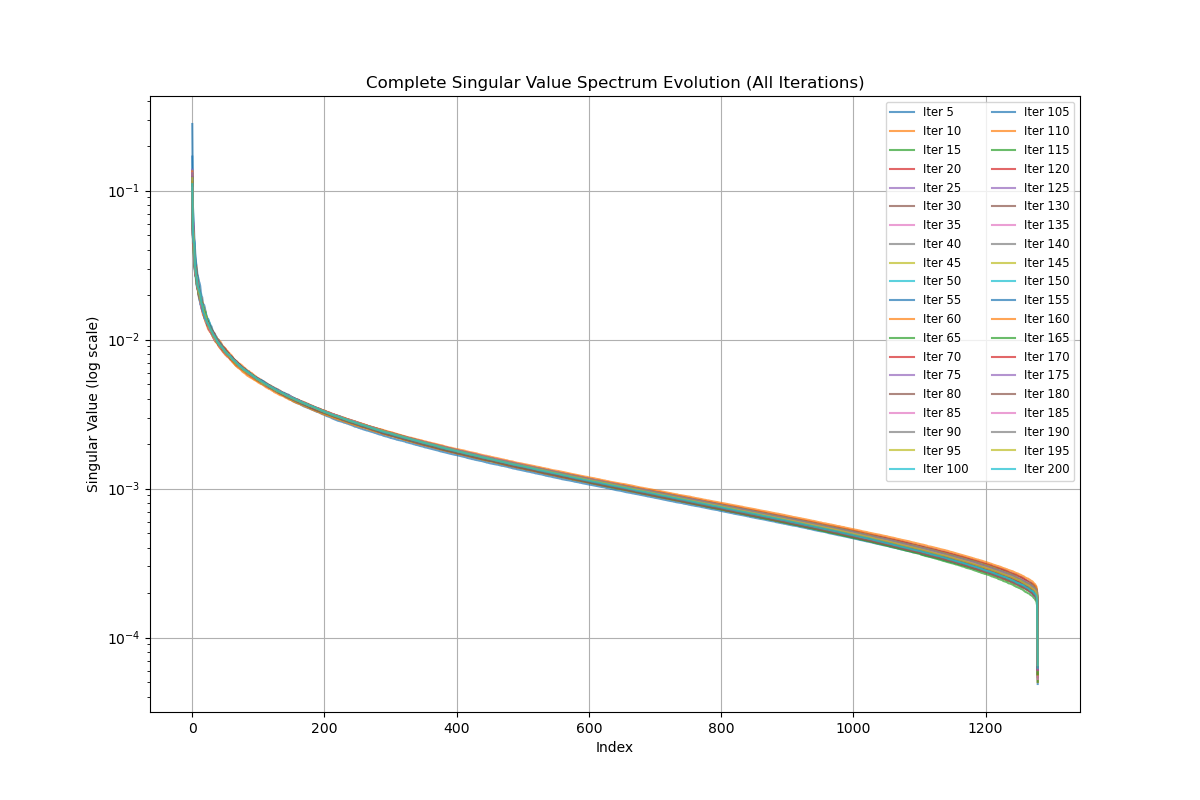
\includegraphics[width=0.8\linewidth]{figs/mlp24/svd_evolution_all.png}}
        \caption{Singular values of $50257\times 1280$ layer via 200 iterations}
        \label{fig:svd_all}
    \end{figure}
    \begin{figure}[h!]
        \center{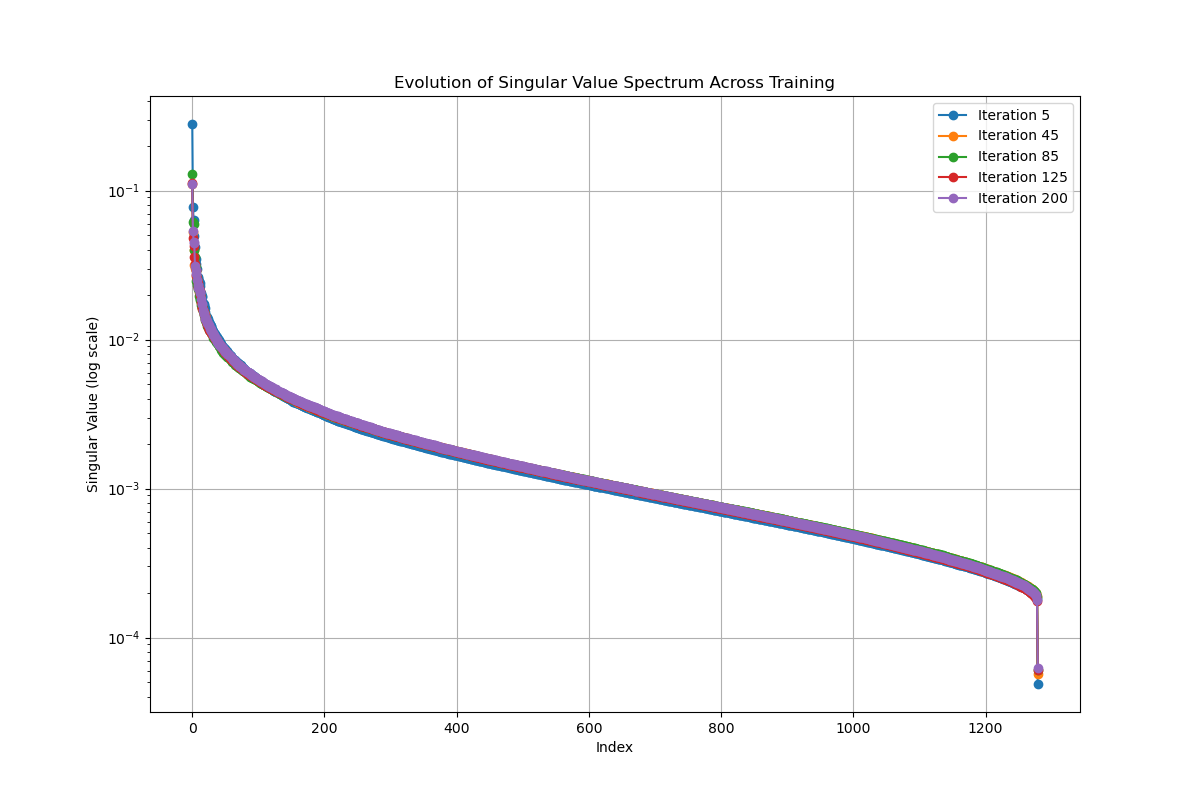
\includegraphics[width=0.8\linewidth]{figs/mlp24/svd_evolution.png}}
        \caption{Singular values of  of $50257\times 1280$ layer for 5-th,45-th, 65-th,175-th and 200-th iteration}
        \label{fig:svd}
    \end{figure} 
    
    \item NanoGPT is tested on Muon and Adam. For now, Neon (rank-1 version) does not converge (see Figures ~\ref{fig:train_loss} \ref{fig:val_loss})
    \begin{figure}[h!]
        \center{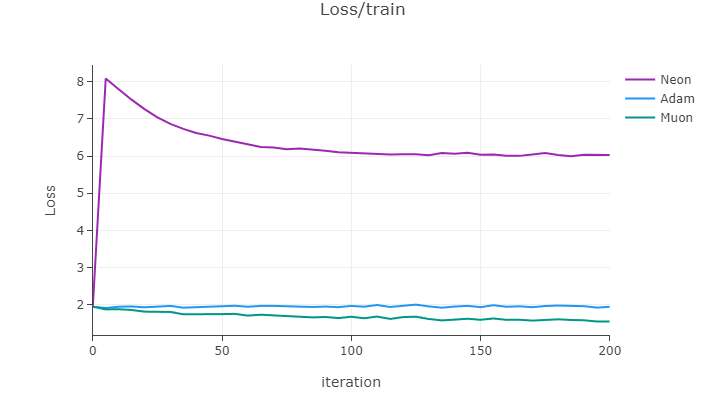
\includegraphics[width=0.8\linewidth]{figs/mlp24/loss_train.png}}
        \caption{Train loss}
        \label{fig:train_loss}
    \end{figure}
    \begin{figure}[h!]
        \center{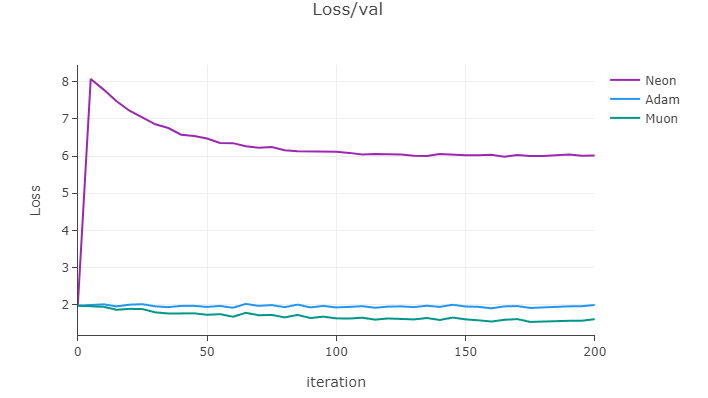
\includegraphics[width=0.8\linewidth]{figs/mlp24/loss_val.png}}
        \caption{Validation loss}
        \label{fig:val_loss}
    \end{figure} 


    The pictures show the best results achieved so far. The experiments were conducted with two 4090 24GB GPUs for nanotgpt-large on the tiny stories dataset.
    
    \item Neon (rank-1 version), Muon, AdamW and SGD are compared on MLP and CNN (see Figures~\ref{fig:mlp_epochs}, \ref{fig:cnn_epochs}, \ref{fig:mlp_time}, and~\ref{fig:cnn_time}). All methods work correctly, but again there is the problem with which one is the fastest (for now, it's SGD).
    \begin{figure}[h!]
        \center{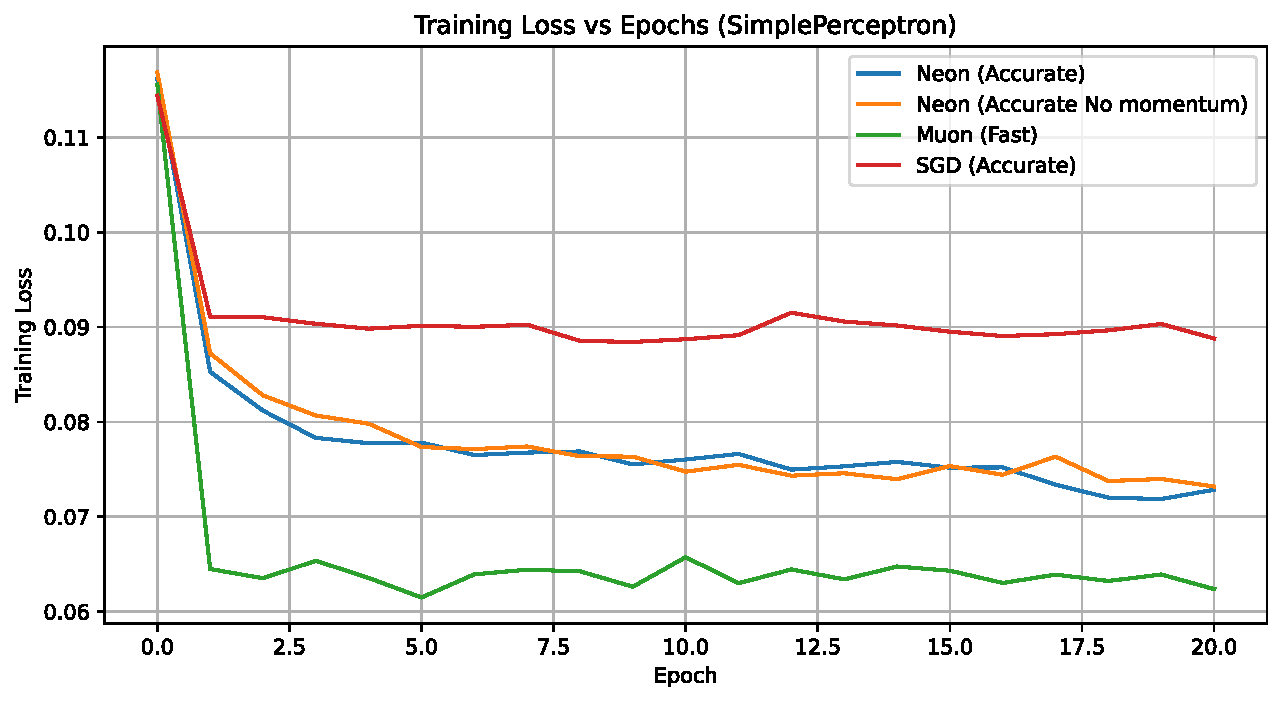
\includegraphics[width=0.8\linewidth]{figs/mlp0605/loss_vs_epochs_mlp.pdf}}
        \caption{MLP: self.linear1 = nn.Linear(32*32*3, 512), self.linear2 = nn.Linear(512, 10), self.activ = nn.GELU()}
        \label{fig:mlp_epochs}
    \end{figure}
    \begin{figure}[h!]
        \center{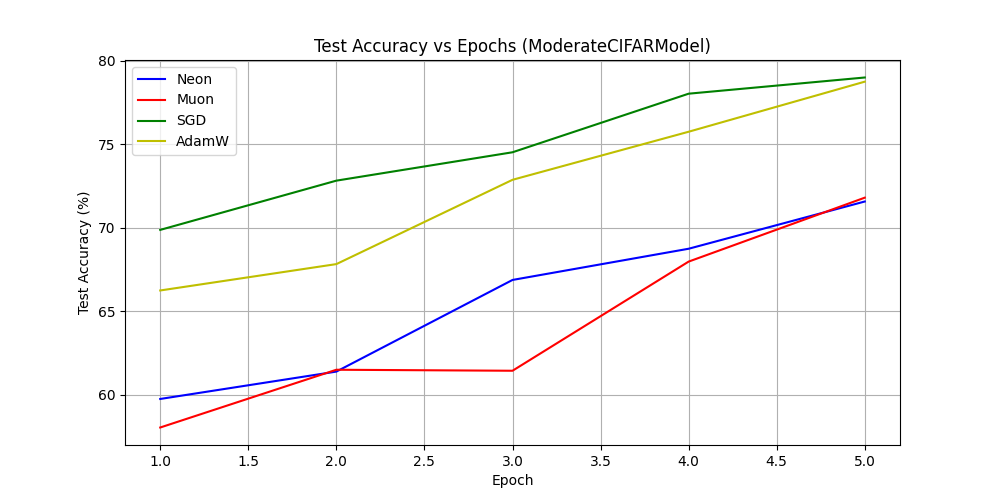
\includegraphics[width=0.8\linewidth]{figs/mlp24/accuracy_vs_epochs_moderate.png}}
        \caption{CNN: 2 convolutional blocks, 2 fully connected layers, activation + dropout}
        \label{fig:cnn_epochs}
    \end{figure}
    \begin{figure}[h!]
        \center{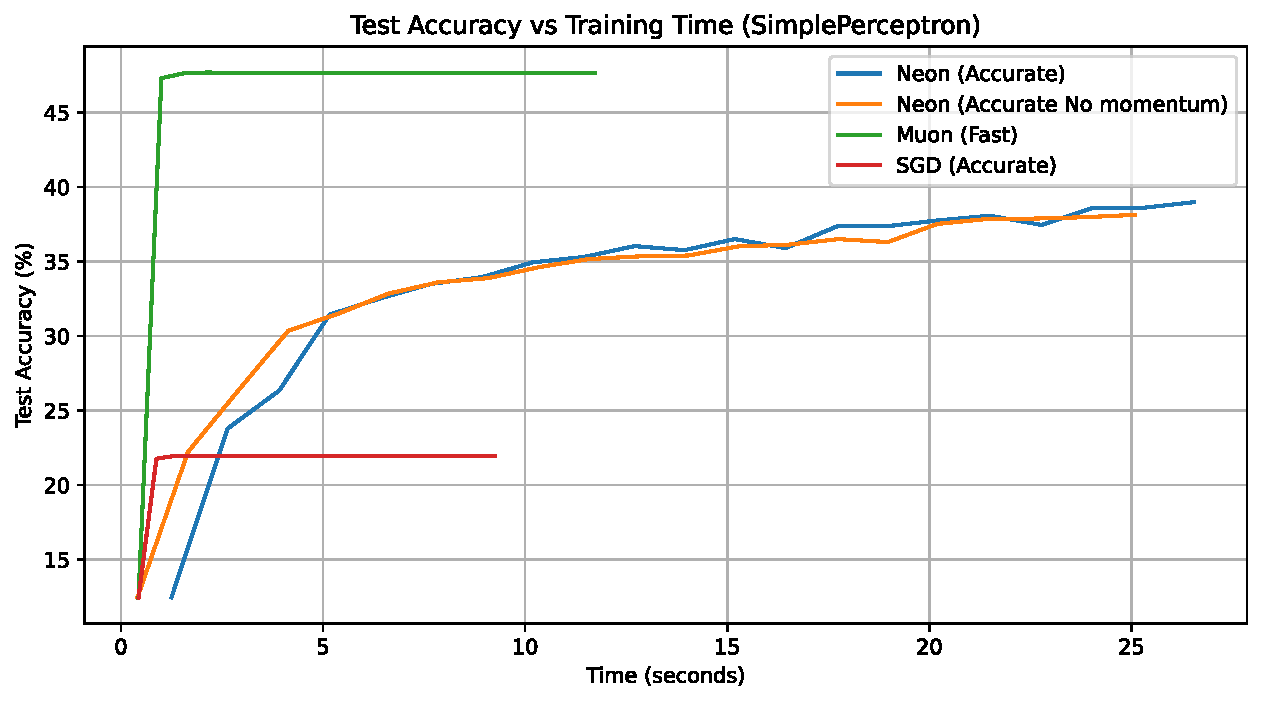
\includegraphics[width=0.8\linewidth]{figs/mlp0605/accuracy_vs_time_mlp.pdf}}
        \caption{MLP: wallclock time measurements}
        \label{fig:mlp_time}
    \end{figure}
    \begin{figure}[h!]
        \center{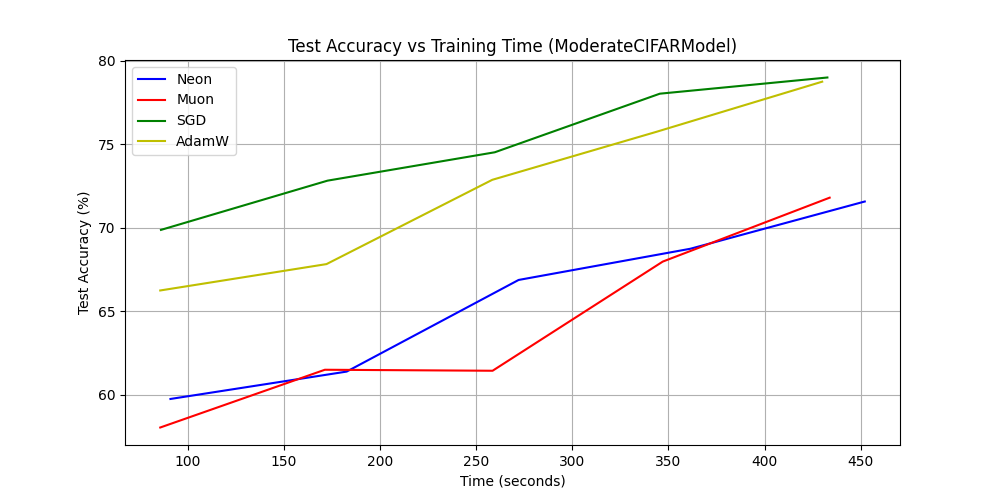
\includegraphics[width=0.8\linewidth]{figs/mlp24/accuracy_vs_time_moderate.png}}
        \caption{CNN: wallclock time measurements}
        \label{fig:cnn_time}
    \end{figure}
    \begin{table}[h!]
        \centering
        \begin{tabular}{c|c|c|c}
        \hline
        Method                              & rtol        & k & time,s \\
        \hline 
        Power Iterations                    & 0.01        & 1 & 7.7\\ 
        SVDS (thick-restart Lanczos method) & 0.01        & 1 & 0.18\\
        PCA Low Rank (RSVD)                 & 0.01        & 1 & 1.15\\
        SVDS (thick-restart Lanczos method) & 0.01        & 10 & 0.47\\
        PCA Low Rank (RSVD)                 & 0.01        & 10 & 19.4\\
        SVDS (thick-restart Lanczos method) & 0.01        & 100 & 1.96\\
        PCA Low Rank (RSVD)                 & 0.01        & 100 & 170\\
        \end{tabular}
        \caption{k-rank updated comparison}
        Comparison of different numerical methods to calculate k-rank update on $5000\times5000$ matrix of real numbers, rtol is an error in Frobenius norm relative to the k-rank approximation of truncated svd. During the research it was noted that rsvd can give good and fast approximation for singular values, but the matrix of approximation is far from the one given by truncated svd, while Lanczos method gives good and fast approximation for a matrix, but not so good approximation for singular values. 
        \label{tab:matrix_methods}
    \end{table}
\end{enumerate}


\appendix
\section{Old Appendix}
You may include other additional sections here.

\fi
\bibliography{icomp2024_conference}
\bibliographystyle{icomp2024_conference}

\end{document}
